%!TEX option = -enable-write18

\documentclass[9pt,xcolor={svgnames, x11names}]{beamer}

\usefonttheme{professionalfonts}
\everymath{\displaystyle}

\usepackage[absolute,overlay]{textpos}
	\setlength{\TPHorizModule}{1.0cm}
	\setlength{\TPVertModule}{\TPHorizModule}
	\textblockorigin{0.0cm}{0.0cm}  %start all at upper left corner
\usepackage{bm}
\usepackage{verbatim} % for latex code in latex doc
\usepackage{tikz}
	\tikzset{every picture/.append style={line cap=round}}
	\usetikzlibrary{calc} % only works within a path. required for member component. and others?
	% \usetikzlibrary{fpu}
	% \usetikzlibrary{math} % if then else etc.
	\usetikzlibrary{arrows.meta}
	% \usetikzlibrary{shadings}
	% \usetikzlibrary{intersections}
	\usetikzlibrary{backgrounds}
\usepackage{pgfmath}

% counter for resuming enumerated list numbers
\newcounter{resumeenumi}
\newcommand{\suspend}{\setcounter{resumeenumi}{\theenumi}}
\newcommand{\resume}{\setcounter{enumi}{\theresumeenumi}}

\newcounter{saveenumi}
\newcommand{\seti}{\setcounter{saveenumi}{\value{enumi}}}
\newcommand{\conti}{\setcounter{enumi}{\value{saveenumi}}}
\resetcounteronoverlays{saveenumi}


% \newcounter{myexercisecounter}
% \newcommand{\suspendExerciseCounter}{\setcounter{myexercisecounter}{\theenumi}}
% \newcommand{\resumeExerciseCounter}{\setcounter{enumi}{\themyexercisecounter}}

\newcommand\lb{\linebreak}
\newcommand\pars{\par\smallskip}
\newcommand\parm{\par\medskip}
\newcommand\parb{\par\bigskip}

%left flushed minipage
\newcommand{\minit}[2][0.8]{
	\begin{minipage}[t]{#1\columnwidth}
		\raggedright
		#2
	\end{minipage}
}

%left flushed minipage
\newcommand{\mini}[2][0.8]{
	\begin{minipage}[c]{#1\columnwidth}
		\raggedright
		#2
	\end{minipage}
}

% centered minipage with text \raggedright
%\cmini[width]{content}
\newcommand{\cmini}[2][0.8]{
	\begin{center}
		\begin{minipage}{#1\columnwidth}
			\raggedright
			#2
		\end{minipage}
	\end{center}
}

\newcommand{\cfig}[2][1]{% centred, scaled graphic
	\begin{center}
		\includegraphics[scale=#1]{#2}
	\end{center}
}
% figure with tight border for photos
% \cfigb[saitMaroon]{borderwidth with unit}{scale}{image}
\newcommand{\cfigb}[4][structure]{
	% \usepackage{adjustbox}
	\setlength{\fboxrule}{1pt}
	\begin{center}
		\includegraphics[scale=#3, cframe= #1 #2]{#4}
	\end{center}
}
\newcommand{\imgbox}[3]{
	% \setlength{\fboxsep}{12pt}
	\includegraphics[scale=#1, cframe= structure #3]{#2}
}

% get x and y coordinates from a tikz coordinate
%\gettikzxy{A}{\ax}{\ay}
\makeatletter
\providecommand{\gettikzxy}[3]{%
	\tikz@scan@one@point\pgfutil@firstofone#1\relax
	\edef#2{\the\pgf@x}%
	\edef#3{\the\pgf@y}%
}
\makeatother

\definecolor{staticsRed}{RGB}{128, 30, 45}
\definecolor{mucus}{rgb}{0.55,0.53,0.31}
\definecolor{myGreen}{RGB}{0,150,0}
\definecolor{saitPurple}{RGB}{112,40,119}
\definecolor{saitDeepBlue}{RGB}{0, 99, 167}
\definecolor{saitBlue}{rgb}{0, 0.59, 0.85}

\definecolor{DarkKhakiMid}{RGB}{235, 228, 134}


%  \definecolor{saitRed}{RGB}{224,38,37} 

%  \definecolor{khaki}{RGB}{190, 183, 107}
%\definecolor{philpotBlue}{RGB}{13,69,120}
% \definecolor{dRed}{rgb}{0.7,0,0}
% \definecolor{blueGrey}{rgb}{0.4,0.48,0.53}
% \definecolor{white}{rgb}{1,1,1}
% \definecolor{dkgreen}{rgb}{0,0.5,0}
% \definecolor{greenyellow}{rgb}{0.9,0.9,0.5}
% \definecolor{flesh}{rgb}{1, 0.95, 0.8}
% \definecolor{wheat}{rgb}{.96, .87, .70}
% \definecolor{oldlace}{rgb}{.992, .96187, .902}
% \definecolor{snow}{rgb}{1, .98, .98}
% \definecolor{ghostwhite}{rgb}{.973, .973, 1}
% \definecolor{cornsilk}{rgb}{1, .973, .863}
% \definecolor{honeydew}{rgb}{.941, 1, .941}
% \definecolor{lavenderdark}{rgb}{.8, .8, .9529411}
% \definecolor{lavender}{rgb}{.902, .902, .980}
% \definecolor{lightblue}{rgb}{.8, .8, .95}
\definecolor{lightgray}{rgb}{.827, .827, .827}
% \definecolor{lightsteelblue}{rgb}{.690, .769, .871}
% \definecolor{lightturquoise}{rgb}{.686, .933, .933}
% \definecolor{darkgreen}{rgb}{.0, .392, .0}
% \definecolor{yellowgreen}{rgb}{.604, .804, .196}
% \definecolor{vlightblue}{rgb}{.88, .85, .95}
% \definecolor{khaki}{rgb}{.741, .718, .42}
% \definecolor{lightkhaki}{rgb}{1, .96, .7}
% \definecolor{almostwhite}{rgb}{1,.95,1}
% \definecolor{facegreen}{rgb}{.45, .5, .2}
% \definecolor{llllBlueGrey}{rgb}{0.8,0.96,1}
% \definecolor{lllBlueGrey}{rgb}{0.69,0.83,0.92}
% \definecolor{llBlueGrey}{rgb}{0.58,0.69,0.76}
% \definecolor{lBlueGrey}{rgb}{0.48,0.58,0.64}
% \definecolor{blueGrey}{rgb}{0.4,0.48,0.53}
% \definecolor{dBlueGrey}{rgb}{0.33,0.4,0.44}
% \definecolor{ddBlueGrey}{rgb}{0.28,0.33,0.37}
% \definecolor{dddBlueGrey}{rgb}{0.23,0.28,0.31}
% \definecolor{almostBlue}{rgb}{0.985,0.985,1}
% \definecolor{almostGreen}{rgb}{0.9,0.97,0.9}

% \definecolor{almostRed}{rgb}{0.95,0.875,0.8}
%  \definecolor{headerGrey}{RGB}{128,128,128}
%  \definecolor{headerGray}{RGB}{128,128,128}
% \definecolor{dHeaderGrey}{RGB}{96,96,96}
% \definecolor{ddHeaderGrey}{RGB}{64,64,64}
% \definecolor{dddHeaderGrey}{RGB}{32,32,32}
% \definecolor{lHeaderGrey}{RGB}{160,160,160}
% \definecolor{llHeaderGrey}{RGB}{192,192,192}
% \definecolor{lllHeaderGrey}{RGB}{224,224,224}
% \definecolor{philpotBlue}{RGB}{13,69,120}
% \definecolor{drabGreen}{RGB}{156,143,87}
% \definecolor{ground}{RGB}{153,153,51}
% \definecolor{gridLight}{rgb}{0.85,0.85,0.85}
% \definecolor{darkGreen}{rgb}{0,0.5,0}

% !TEX root = ../../statikz/statikz.tex

% % get x and y coordinates from a tikz coordinate, returned values in points
% \makeatletter
% \providecommand{\gettikzxy}[3]{%
%   \tikz@scan@one@point\pgfutil@firstofone#1\relax
%   \edef#2{\the\pgf@x}%
%   \edef#3{\the\pgf@y}%
% }
% \makeatother

%\Member{startpt}{endpt}{outer}{inner}{stroke}{height}{radius}{line width}
\providecommand{\Member}[8]{

  \def\topt{28.45274}
  \def\tocm{0.035146}
  % name the points
  \coordinate (start) at (#1); % coordinate
  \coordinate (end) at (#2); % coordinate
  
  \def\outer{#3} % color
  \def\inner{#4} % color
  \def\stroke{#5} % color
  \def\hi{#6} % cm
  \def\rad{#7} % cm
  \def\line{#8} % mm
  
  \gettikzxy{(start)}{\sx}{\sy}
  \gettikzxy{(end)}{\ex}{\ey}
  
  \coordinate(delta) at ($ (end)-(start) $);
  \gettikzxy{(delta)}{\dx}{\dy}
  
  \pgfmathparse{veclen(\dx, \dy)}% \pgfmathresult
  \let\length\pgfmathresult
  
  \pgfmathparse{\dx==0}%
  % \ifnum low-level TeX for integers
  \ifnum\pgfmathresult=1 % \dx == 0
    \pgfmathsetmacro{\rot}{\dy > 0 ? 90 : -90}
  \else
    \pgfmathsetmacro{\rot}{\dx > 0 ? atan(\dy / \dx) : 180 + atan(\dy / \dx)}
    
  \fi
  
  \fill[\inner] (#1) circle (.1mm); % node[black] {\sx, \sy};
  \fill[\inner] (#2) circle (.1mm); % node[black] {\ex, \ey};
  \begin{scope}	[rounded corners = 0.9*\rad cm, transform canvas = {rotate around = {\rot:(start)}}]
    \shadedraw[top color = \outer, bottom color = \outer, middle color = \inner, draw = \stroke, line width = \line mm] ($ (start)+(-0.5*\hi, 0.5*\hi) $) -- ++(\hi cm +\length pt, 0 ) -- ++(0, -\hi) -- ++ (-\hi cm -\length pt, 0) -- cycle;    
  \end{scope}
  
  % \draw[black] (start) circle (2mm);
  % \draw[black] (end) circle (2mm);
}


\newcommand{\PinnedConnection}[6][0]{
	\def\lrotate{#1}
	\def\lpin{#2}
	\def\lfill{#3}
	\def\ldraw{#4}
	\def\lscale{#5}
	\def\lwidth{#6}
	\def\h{1}
	\def\r{0.3}
	\begin{scope}[scale=\lscale, rotate=\lrotate]
		\filldraw[draw=\ldraw, fill=\lfill, line width=\lwidth mm] ($(\lpin) + (0.201*\h+1.0353*\r ,-0.75*\h)$) -- ++(105: 0.77646*\h+0.26795*\r) arc (15:165:\r) -- ++(-105:0.77646*\h+0.26795*\r) -- cycle;
		
		% \shadedraw[ball color=\lfill, draw=\ldraw, line width = \lwidth mm] (\lpin) circle (1.5mm);
		
		\filldraw[rounded corners=\lscale pt, draw=\ldraw, fill=\lfill, line width=\lwidth mm] ($ (\lpin) - (1,1) $) rectangle +(2,0.35);
	\end{scope}
}


\hypersetup{
	colorlinks,
	linkcolor=staticsRed, % table of contents
	urlcolor=staticsRed
}

\usetheme{Antibes}
\usecolortheme[named=staticsRed]{structure}
\setbeamertemplate{blocks}[rounded][shadow=false]
\setbeamertemplate{headline}{\vspace{.1cm}}
\setbeamertemplate{navigation symbols}{} % empty braces suppresses all navigation symbols
\setbeamertemplate{footline}{
  \hfill
  \insertshorttitle
  \quad
  \insertsection
  \quad
  \insertsubsection
  \quad
  \insertframenumber/\inserttotalframenumber
  \quad{ }
  \vspace{0.125cm}
}
\addtobeamertemplate{footline}{\hypersetup{linkcolor=black}}{}
\setbeamertemplate{navigation symbols}{} % empty braces suppresses all navigation symbols
% \setbeamercolor{frametitle}{fg=white}
\setbeamertemplate{section in toc shaded}[default][50]
% \setbeamertemplate{subsection in toc}[subsections numbered]
\setcounter{tocdepth}{5}

% various hacks to get around (apparent?) Beamer titlepage constraints
\title[\color{black} Statikz \textcolor{Maroon}{ (2020-\the\year)}]{\Huge Statikeetz}
\subtitle{} % i.e., a blank line
\institute{\small Source code at: \lb{\footnotesize\url{https://github.com/dmorgorg/LaTeX2022}}}
\author{} % another blanky
\date{\small Last updated on \today}

%%%%%%%%%%%%%%%%%%%%%%%%%%%%%%%%%%%%%%%%%%%%%%%%%%%%%%%%%%%%%%%%%%%%%%%%%%%%%%%%%%%%%%%%%%%%%%%%%%%%%%%%%%%%%%
\begin{document}
%%%%%%%%%%%%%%%%%%%%%%%%%%%%%%%%%%%%%%%%%%%%%%%%%%%%%%%%%%%%%%%%%%%%%%%%%%%%%%%%%%%%%%%%%%%%%%%%%%%%%%%%%%%%%%
\begin{frame}
	\titlepage
\end{frame}

\begin{frame}{Table of Contents}
	\begin{minipage}{0.9\textwidth}
		\tableofcontents
	\end{minipage}
	\vfill
\end{frame}

%%%%%%%%%%%%%%%%%%%%%%%%%%%%%%%%%%%%%%%%%%%%%%%%%%%%%%%%%%%%%%%%%%%%%%%%%%%%%%%%%%%%%%%%%%%%%%%%%%%%%%%%%%%%%%
\section{Tikz Drawing Components}
\centering  % centres all components, pikz on the frame
%%%%%%%%%%%%%%%%%%%%%%%%%%%%%%%%%%%%%%%%%%%%%%%%%%%%%%%%%%%%%%%%%%%%%%%%%%%%%%%%%%%%%%%%%%%%%%%%%%%%%%%%%%%%%%
\begin{frame}[fragile]{Tikz Components :: Member}

	\small
	\begin{verbatim}
		\Member{startpt}{endpt}{outer}{inner}{stroke}{height}{radius}{line width}
		 \end{verbatim}
	\parb
	% \vspace{2cm}
		%  \centering
	\resizebox{0.75\textwidth}{!}{%
		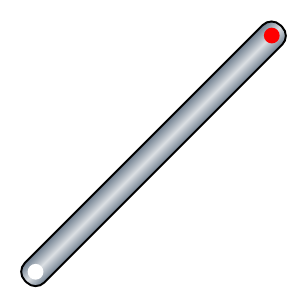
\begin{tikzpicture}
			\coordinate (A) at (0,0);
			\coordinate (B) at (3,3);
			\coordinate (C) at (8,0);
			\coordinate (D) at (6,-0.5);
			\coordinate (E) at (2,0.5);
			\Member{A}{B}{SlateGray}{SlateGray!25!white}{black}{0.35}{0.175}{.25}
			\fill[white] (A) circle (1mm);
			\fill[red] (B) circle (1mm);
		\end{tikzpicture}

	}
\end{frame}
%%%%%%%%%%%%%%%%%%%%%%%%%%%%%%%%%%%%%%%%%%%%%%%%%%%%%%%%%%%%%%%%%%%%%%%%%%%%%%%%%%%%%%%%%%%%%%%%%%%%%%%%%%%%%%
\begin{frame}[fragile]{Tikz Components :: Member}

	\small\centering
	\begin{verbatim}
		\Member{startpt}{endpt}{outer}{inner}{stroke}{height}{radius}{line width}
		 \end{verbatim}
	\parb
	% \vspace{2cm}

	\resizebox{0.75\textwidth}{!}{%
		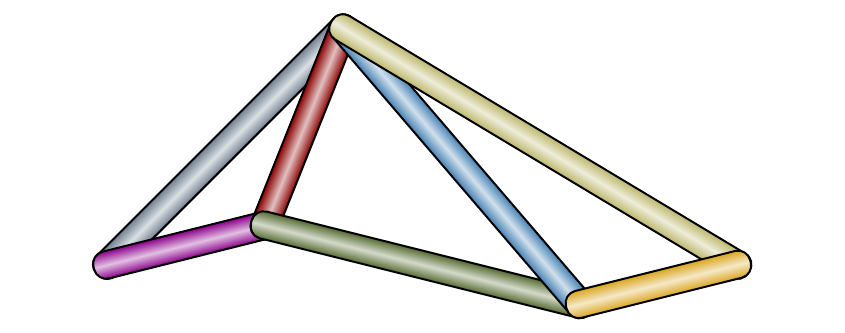
\begin{tikzpicture}
			\coordinate (A) at (0,0);
			\coordinate (B) at (3,3);
			\coordinate (C) at (8,0);
			\coordinate (D) at (6,-0.5);
			\coordinate (E) at (2,0.5);
			\Member{A}{B}{SlateGray}{SlateGray!25!white}{black}{0.35}{0.175}{.25}
			\Member{A}{E}{DarkMagenta}{DarkMagenta!25!white}{black}{0.35}{0.175}{.25}
			\Member{E}{B}{DarkRed}{DarkRed!25!white}{black}{0.35}{0.175}{.25}
			\Member{E}{D}{DarkOliveGreen}{DarkOliveGreen!25!white}{black}{0.35}{0.175}{.25}
			\Member{D}{B}{SteelBlue}{SteelBlue!25!white}{black}{0.35}{0.175}{.25}
			\Member{C}{B}{DarkKhaki}{DarkKhaki!25!white}{black}{0.35}{0.175}{.25}
			\Member{D}{C}{Goldenrod}{Goldenrod!25!white}{black}{0.35}{0.175}{.25}
			\fill[white] (-1,0) circle (0.1mm);
			\fill[white] (9,0) circle (0.1mm);
		\end{tikzpicture}

	}
\end{frame}

%%%%%%%%%%%%%%%%%%%%%%%%%%%%%%%%%%%%%%%%%%%%%%%%%%%%%%%%%%%%%%%%%%%%%%%%%%%%%%%%%%%%%%%%%%%%%%%%%%%
\begin{frame}[fragile]{Tikz Components :: PinnedConnection}

	\small
	\begin{verbatim}
	  \PinnedConnection[rotate=0]{coordinate}{fill}{draw}{scale}{line width}
  	\end{verbatim}
	\vspace{1cm}
	\tikz{
		\coordinate (A) at (0,0);
		% \PinnedConnection[rotate=0]{coordinate}{fill}{draw}{scale}{line width}
		\PinnedConnection{A}{Honeydew1}{Black}{2}{0.5}
	}

\end{frame}

%%%%%%%%%%%%%%%%%%%%%%%%%%%%%%%%%%%%%%%%%%%%%%%%%%%%%%%%%%%%%%%%%%%%%%%%%%%%%%%%%%%%%%%%%%%%%%%%%%%
\section{06 Equilibrium of Rigid Bodies}
%%%%%%%%%%%%%%%%%%%%%%%%%%%%%%%%%%%%%%%%%%%%%%%%%%%%%%%%%%%%%%%%%%%%%%%%%%%%%%%%%%%%%%%%%%%%%%%%%%%
\begin{frame}
	\def\scale{0.7}
	\tikz[scale=\scale]{
    \coordinate (A) at (0,0);
    \coordinate (B) at (8,0);
    \coordinate (C) at (2,2.5);
    \coordinate (BCmid) at ($(B)!0.5!(C)$);

    \gettikzxy{(A)}{\ax}{\ay}
    \gettikzxy{(B)}{\bx}{\by}
    \gettikzxy{(C)}{\cx}{\cy}
    \gettikzxy{(BCmid)}{\bcmidx}{\bcmidy}

    % \filldraw[fill=white, draw=red, opacity=0.75] ($(A)+(-2.75,-2.75)$) rectangle (\bx+1.75cm, \cy+1.75cm);

    \PinnedConnection{A}{DarkOliveGreen4}{black}{0.5}{0.125}
    \PinnedConnection{B}{DarkOliveGreen4}{black}{0.5}{0.125}
    \shade[top color=Ivory4, bottom color= white] ($(A)+(-2,-0.5)$) rectangle ($(B)+(1,-1.5)$);
    \draw[Ivory4!50!black] ($(A)+(-2,-0.5)$) -- ($(B)+(1,-0.5)$);

    \def\delta{0.175}
    \def\left{-1.75}
    \def\bot{-1.75}
    \def\bottom{-2}
    \filldraw[fill=Ivory3, draw=black] ($(A)+(-\delta,0)$)--(\ax-\delta cm, \cy-\delta cm)arc(180:90:2*\delta cm)--(\cx,\cy+\delta cm)arc(90:-90:\delta)--(\ax+2*\delta cm, \cy-\delta cm)arc(90:180:\delta)--(\ax+\delta cm, \ay)arc(360:180:\delta);
    \Member{B}{C}{Ivory3}{Ivory3}{black}{0.35}{0.175}{.125}

    \filldraw[ball color=Ivory4, draw=Ivory4!50!black, thin] (A) circle (1mm);
    \filldraw[ball color=Ivory4, draw=Ivory4!50!black, thin] (B) circle (1mm);
    \filldraw[ball color=Ivory4, draw=Ivory4!50!black, thin] (C) circle (1mm);
    \filldraw[color=white, draw=black, thin] (BCmid) circle (0.5mm);

    \draw (A)  node[black, left, inner sep=5pt] {$A$};
    \draw (B)  node[black, above right, inner sep=3.5pt] {$B$};
    \draw (C)  node[black, above right, inner sep=4pt] {$C$};

    \draw[very thick, Latex-, saitDeepBlue] ($(B)!0.5!(C)$)--+(0,2)node[above, black]{$10.0\,\text{kN}$ };
    \draw[very thin] ($(A)+(0.5,0)$)--($(B)+(-0.875,0)$);
    \draw[very thin] ($(A)+(-0.75,0)$)--(\left,\ay);
    \draw[very thin] ($(C)+(-0.5,0)$)--(\left,\cy);
    \draw[very thin] (\ax+0.5cm,\cy)--($(C)+(-0.5,0)$);
    \draw[very thin] (\ax,\ay-0.25cm)--(\ax, \bottom);
    \draw[very thin] (\bx,\by-0.25cm)--(\bx, \bottom);
    \draw[very thin] (\cx,\cy-0.375cm)--(\cx, \bottom);
    \draw[very thin] (\bcmidx, \bcmidy-0.375cm)--(\bcmidx, \bottom);

    \small
    \draw[latex-latex] (\ax,\bot)--node[fill=white, inner sep=0.5mm]{$1.00\,\text{m}$}(\cx,\bot);
    \draw[latex-latex] (\cx,\bot)--node[fill=white, inner sep=0.5mm]{$1.50\,\text{m}$}(\bcmidx,\bot);
    \draw[latex-latex] (\bcmidx,\bot)--node[fill=white, inner sep=0.5mm]{$1.50\,\text{m}$}(\bx,\bot);
    \draw[latex-latex] (\ax-1.5cm,\cy)--node[fill=white, inner sep=0.5mm]{$1.25\,\text{m}$}(\ax-1.5cm,\ay);



}
\end{frame}


%%%%%%%%%%%%%%%%%%%%%%%%%%%%%%%%%%%%%%%%%%%%%%%%%%%%%%%%%%%%%%%%%%%%%%%%%%%%%%%%%%%%%%%%%%%%%%%%%%%
\section{09 Frames}
%%%%%%%%%%%%%%%%%%%%%%%%%%%%%%%%%%%%%%%%%%%%%%%%%%%%%%%%%%%%%%%%%%%%%%%%%%%%%%%%%%%%%%%%%%%%%%%%%%%
\begin{frame}
	hello
\end{frame}

%%%%%%%%%%%%%%%%%%%%%%%%%%%%%%%%%%%%%%%%%%%%%%%%%%%%%%%%%%%%%%%%%%%%%%%%%%%%%%%%%%%%%%%%%%%%%%%%%%%
\end{document}
%%%%%%%%%%%%%%%%%%%%%%%%%%%%%%%%%%%%%%%%%%%%%%%%%%%%%%%%%%%%%%%%%%%%%%%%%%%%%%%%%%%%%%%%%%%%%%%%%%%
